\documentclass[12pt,twocolumn]{article}
\usepackage[utf8]{inputenc}
\usepackage[english]{babel}
\usepackage[table,xcdraw]{xcolor}
\usepackage{physics}
\usepackage{fancyhdr}
\usepackage{geometry}
\usepackage{natbib}
\usepackage{graphicx}
\usepackage{float}
\usepackage{wrapfig}
%\usepackage{caption}
\usepackage[justification=centering]{caption}
\usepackage{subcaption}
\usepackage{gensymb}
\usepackage[export]{adjustbox}
\usepackage{hyperref}
\geometry{margin = 20mm}
\usepackage{mathtools}
\usepackage{amsmath}
\usepackage{indentfirst}
\usepackage{xurl}
\usepackage{t1enc}
\usepackage{setspace}



\title{Simulating detectors with Geant4}
\author{Scientific Modeling Computer Laboratory\\Bendegúz Borkovits T7UR9P\\Supervisor: Ákos Horváth}
\date{March 2022}


\begin{document}

\maketitle

\section{Introduction}

Geant4 is a software developed at CERN. Its main purpose is to allow the user to create virtual detectors to simulate and visualize the interaction of particles with each other and with the defined detector. The software provides a large variety in parameters for the simulations such as parameters that define the geometry of a detector and its material properties, the laws of physics that will be enabled in the proximity of said detector and many more.

The long-term aim of the project is to model a neutron detector. The parameters of said detector will be provided later by the supervisor. Up until the creation of this report, my task consisted of following tutorials \cite{youtube} and the documentation \cite{geant} of the software to be able to grasp the knowledge on how a simulation in Geant4 could be created. To learn the steps of programming a simulation, I have followed a series of tutorial lectures that aimed toward creating a program that was centered around the appearance of Cherenkov radiation and detecting the resulting optical photons in the process.

\section{Building a simulation}

A simulation in Geant4 is a Cmake project, therefore, naturally one needs to start building it by defining its Cmake properties. Geant4 allows support for tools and environments such as Qt5 and Python, it also offers a multi-threading mode, though in this project everything was done in single-threading mode in order not to run into a few problems regarding multi-threading and its effect on the simulations. Geant4 offers support for various operating systems such as Ubuntu and Windows. It should be noted that the Windows version runs considerably slower than its Linux counterpart, therefore in this project Ubuntu 18.04 was used as the environment. Said operating system was used as a virtual machine, set up in the Oracle VM VirtualBox application. Although, 18.04 is not the newest version of Ubuntu, it seemed to be more stable when started from VirtualBox than the newer versions.

After setting up the environment and the respective Cmake files, I started to define structure of the simulation. To make the project seem more organized, one should divide the program into individual parts according to their respective purpose. Firstly, the main function of the simulation was defined and contained int the file \emph{sim.cc}. Said function consists of the executive commands and some refinement commands for the visualization. Then, defining the geometry should be the next part in the process. This step of the simulation is contained in the files \emph{construction.cc} and \emph{construction.hh}. First, one should declare the shape and size of the world itself. In this case, the world volume is simply a box with the width, length and height of one meter. The logical and physical parameters of the world consist of it having air inside of it and having the origin of the coordinate system in its centre. After that, one should create a desired detector. The parameters of said detector are made up by its geometry and material properties. In Geant4, one is able to create complex molecules by defining and combining simpler molecules. To this end, I built up silicon-dioxide, water and carbon molecules to combine them into an aerogel detector that consist of the following percentages of the previously mentioned molecules: 62.6\%, 37.4\% and 0.1\%. Finally, I defined the shape of the detector as a smaller box with considerably smaller length than width and height and placed it inside the world volume. It should be noted that the different sizes of the detector always need to be smaller than that of the world volume.

As a next step, one should generate a few particles. In this project the G4ParticleGun class was used as a generator. To test whether this method works, I generated a proton with a Z-directional momentum of 100 GeV that goes through the centre of the detector. the properties of said proton were defined in files \emph{generator.cc} and \emph{generator.hh}. For computing purposes, one should define an action manager that manages the process of particle generating. This part of the simulation is included in \emph{action.cc} and \emph{action.hh}.

\begin{figure}[H]
    \centering
    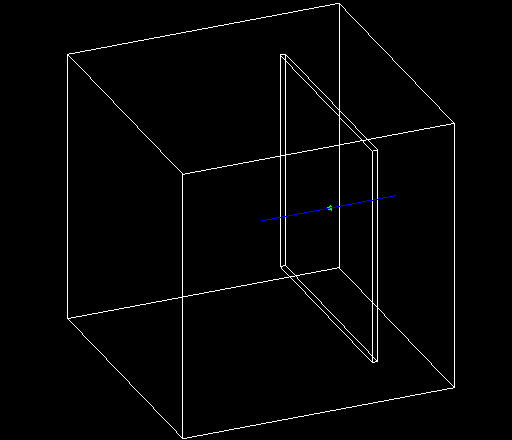
\includegraphics[scale=0.64]{detector_volume.png}
    \caption{The box shaped detector contained within the world volume. The blue line indicates the defined proton and the green line indicates the optical photons that were produced via Cherenkov radiation. Sometimes red lines also appear, indicating the presence of $\beta$-electrons.}
    \label{fig:basic}
\end{figure}

The final step in completing the simulation is creating a suitable physics list, in this case enabling the occurrence of optical photons and the existence of electromagnetic interaction. The code of this step is located in files \emph{physics.cc} and \emph{physics.hh}. The result is showcased on Figure 1. The proton collides and goes through the detector, while optical photons are produced upon entry as Cherenkov radiation.

\section{Detecting photons}

In order to inquire information about the optical photons, they need to propagate through the aerogel detector and collide with a wall made of small sensitive detectors. To that end, one needs to define the refractive indices of the aerogel detector and the world volume separately. Then, one should include the properties of the photo-sensitive detectors into the simulation. The material properties and geometry were defined in the file \emph{construction.cc}. Essentially, I created a wall that has a small detector for every segment and each of these can detect an incoming photon. Finally, one needs to precisely tell the program, what kind of information one would like to gain. As an easier example, I have asked information about the positions where the photons enter the wall of sensitive detectors. The resulting data consisted of the position of the side of the detector that was closer to the aerogel box. The declarations of this information can bee seen in files \emph{detector.cc} and \emph{detector.hh}.

Saving the output of a Geant4 simulation is relatively straight forward. One needs to create several columns to separate the different datasets and fill them with the yielded results. There are four file formats one can work with regarding Geant4. These are the following: ROOT, CSV, XML and HBOOK. ROOT seems to be the favoured method for working with Geant4 and to that end, I have installed the ROOT software to test the accessibility of said format. In the end, working with CSV files turned out to be the more favourable option, as I was planning to evaluate my data using Python and the NumPy module provides user friendly methods to deal with CSV files. Saving the output requires the creation of a run manager that manages all the saving commands and works with the built-in library of the chosen file format, such as g4csv. The run manager was put into the files \emph{run.cc} and \emph{run.hh}.

\begin{figure}[H]
    \centering
    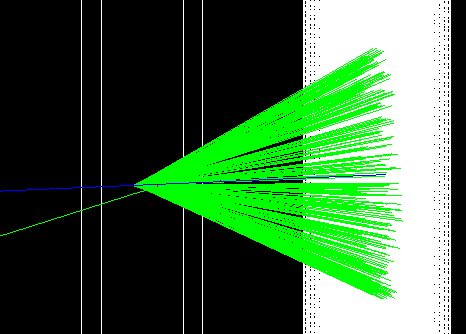
\includegraphics[scale=0.8]{sensitive_detectors.png}
    \caption{The proton (blue) produces the cone of photons (green) when going through the aerogel detector and the photons reach the sensitive detectors (white). The tiny red line indicates a $\beta$-electron. The one photon on the other side of the detector is some back scattering event that occurs with very low probability.}
    \label{fig:my_label}
\end{figure}

\section{Showcasing the output}

To plot the positions, where the photons entered the wall of detectors, I used matplotlib.pyplot in a Jupyter notebook. To generate data, I saved ten events of Cherenkov radiation caused by a proton, meaning that I ran the simulation ten separate times and stored the information yielded by each run in a single file. Then, I checked the distribution of the number of photons generated by each event. The result is showcased on Figure 3. It can be seen that each run generates almost the same number of photons with a mean of $308\pm17$ particles. Then, I plotted the XY-coordinates of each data point and checked whether or not the extraction of the results was successful by expecting a circle to be formed. The result can be seen on Figure 4.

\begin{figure}[H]
    \centering
    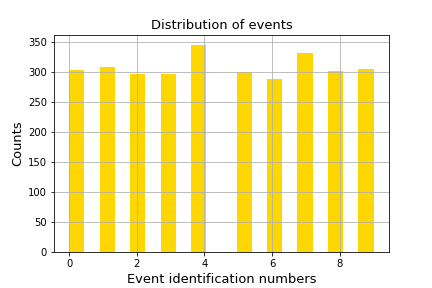
\includegraphics[scale=0.65]{histo.png}
    \caption{Showing the amount of photons generated by each individual run. They showcase a rather uniform distribution.}
    \label{fig:my_label}
\end{figure}
\begin{figure}[H]
    \centering
    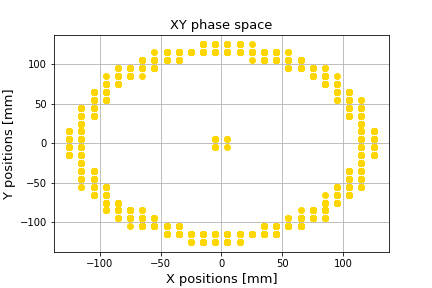
\includegraphics[scale=0.65]{xy_phase.png}
    \caption{Showcasing the positions of the photons upon entry to the sensitive detector wall on the XY-plane.}
    \label{fig:my_label}
\end{figure}

On Figure 4, one can indeed view the circular shape, however four data points were shown in the middle of the figure. This is once again due to the occurrence of some sort of low probability scattering event that places a photon in the run that it happens in the middle of the figure. The evidence that suggest this are the facts that the proton does not interact with the sensitive detectors and this happens only four times out of ten runs. The evaluation of the data can be found in file \emph{analysis.ipynb}.

\section{Discussion}

In the first half of project, I have studied how to build up a simulation in Geant4. To that end, I followed a series of tutorials from a Youtube channel under the name of Physics Matters \cite{youtube} to create the simulation of the above explained Cherenkov radiation. While completing the tutorials, I have learnt about the stepping stones and the parameter space of such a model, as well as acquired the means to extract and evaluate the data yielded by the simulation, to prepare myself for the next part of the project, modelling a neutron detector and build its code from scratch.

A few technical difficulties occurred while working on the simulation that are worth discussing, should someone experience them in the future. It has already been discussed that using Ubuntu 18.04 instead of an older version on VirtualBox is a fairly good idea due to reasons of stability. Similar issues as well as compatibility issues might also arise when dealing directly with Geant4. For example, in this project, the optical photons only appeared on Figure 1 when using the 10.7.03 version instead of the newer 11 version. As I have seen it on the Internet, this seemed to be a reoccurring problem regarding optical photons. Finally, a strange issue has surfaced when I saved the output of the simulation into a CSV file. The data, I planned to extract, was saved into an additional file, while the original output file only contained the defined headers. Although, this problem does not cause any errors that compromise saving data, it is still out of the ordinary and might have been caused by a bug related to the g4csv package.


\bibliographystyle{plain}
\bibliography{references.bib}




\end{document}
